% Created by tikzDevice version 0.7.0 on 2014-07-24 03:38:09
% !TEX encoding = UTF-8 Unicode
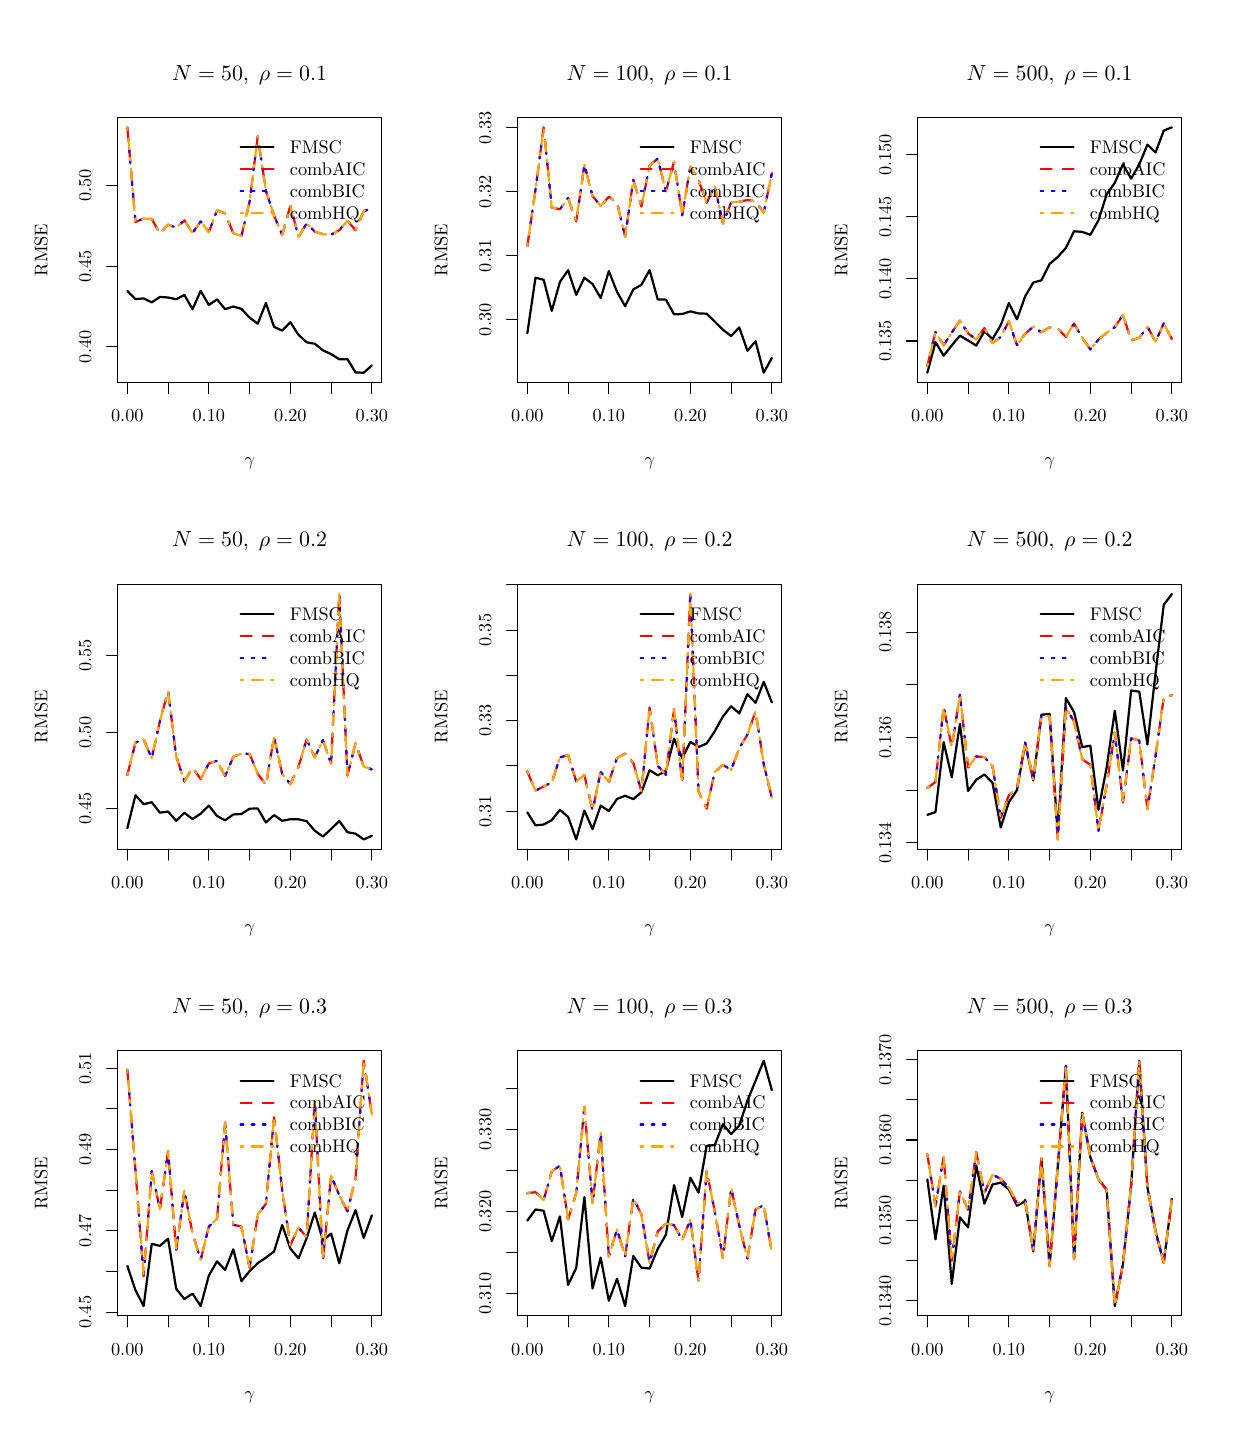
\begin{tikzpicture}[x=1pt,y=1pt]
\definecolor[named]{fillColor}{rgb}{1.00,1.00,1.00}
\path[use as bounding box,fill=fillColor,fill opacity=0.00] (0,0) rectangle (433.62,505.89);
\begin{scope}
\path[clip] ( 32.47,377.65) rectangle (127.91,473.42);
\definecolor[named]{drawColor}{rgb}{0.00,0.00,0.00}

\path[draw=drawColor,line width= 0.8pt,line join=round,line cap=round] ( 36.01,410.73) --
	( 38.95,407.81) --
	( 41.90,408.04) --
	( 44.84,406.63) --
	( 47.79,408.59) --
	( 50.73,408.38) --
	( 53.68,407.77) --
	( 56.63,409.31) --
	( 59.57,404.15) --
	( 62.52,410.78) --
	( 65.46,405.66) --
	( 68.41,407.70) --
	( 71.35,404.16) --
	( 74.30,405.12) --
	( 77.24,404.27) --
	( 80.19,401.10) --
	( 83.14,398.90) --
	( 86.08,406.37) --
	( 89.03,397.77) --
	( 91.97,396.40) --
	( 94.92,399.45) --
	( 97.86,394.89) --
	(100.81,392.20) --
	(103.75,391.67) --
	(106.70,389.28) --
	(109.65,387.92) --
	(112.59,386.07) --
	(115.54,386.11) --
	(118.48,381.30) --
	(121.43,381.20) --
	(124.37,383.84);
\end{scope}
\begin{scope}
\path[clip] (  0.00,  0.00) rectangle (433.62,505.89);
\definecolor[named]{drawColor}{rgb}{0.00,0.00,0.00}

\path[draw=drawColor,line width= 0.4pt,line join=round,line cap=round] ( 36.01,377.65) -- (124.37,377.65);

\path[draw=drawColor,line width= 0.4pt,line join=round,line cap=round] ( 36.01,377.65) -- ( 36.01,373.69);

\path[draw=drawColor,line width= 0.4pt,line join=round,line cap=round] ( 50.73,377.65) -- ( 50.73,373.69);

\path[draw=drawColor,line width= 0.4pt,line join=round,line cap=round] ( 65.46,377.65) -- ( 65.46,373.69);

\path[draw=drawColor,line width= 0.4pt,line join=round,line cap=round] ( 80.19,377.65) -- ( 80.19,373.69);

\path[draw=drawColor,line width= 0.4pt,line join=round,line cap=round] ( 94.92,377.65) -- ( 94.92,373.69);

\path[draw=drawColor,line width= 0.4pt,line join=round,line cap=round] (109.65,377.65) -- (109.65,373.69);

\path[draw=drawColor,line width= 0.4pt,line join=round,line cap=round] (124.37,377.65) -- (124.37,373.69);

\node[text=drawColor,anchor=base,inner sep=0pt, outer sep=0pt, scale=  0.66] at ( 36.01,363.40) {0.00};

\node[text=drawColor,anchor=base,inner sep=0pt, outer sep=0pt, scale=  0.66] at ( 65.46,363.40) {0.10};

\node[text=drawColor,anchor=base,inner sep=0pt, outer sep=0pt, scale=  0.66] at ( 94.92,363.40) {0.20};

\node[text=drawColor,anchor=base,inner sep=0pt, outer sep=0pt, scale=  0.66] at (124.37,363.40) {0.30};

\path[draw=drawColor,line width= 0.4pt,line join=round,line cap=round] ( 32.47,390.54) -- ( 32.47,448.79);

\path[draw=drawColor,line width= 0.4pt,line join=round,line cap=round] ( 32.47,390.54) -- ( 28.51,390.54);

\path[draw=drawColor,line width= 0.4pt,line join=round,line cap=round] ( 32.47,419.66) -- ( 28.51,419.66);

\path[draw=drawColor,line width= 0.4pt,line join=round,line cap=round] ( 32.47,448.79) -- ( 28.51,448.79);

\node[text=drawColor,rotate= 90.00,anchor=base,inner sep=0pt, outer sep=0pt, scale=  0.66] at ( 22.97,390.54) {0.40};

\node[text=drawColor,rotate= 90.00,anchor=base,inner sep=0pt, outer sep=0pt, scale=  0.66] at ( 22.97,419.66) {0.45};

\node[text=drawColor,rotate= 90.00,anchor=base,inner sep=0pt, outer sep=0pt, scale=  0.66] at ( 22.97,448.79) {0.50};

\path[draw=drawColor,line width= 0.4pt,line join=round,line cap=round] ( 32.47,377.65) --
	(127.91,377.65) --
	(127.91,473.42) --
	( 32.47,473.42) --
	( 32.47,377.65);
\end{scope}
\begin{scope}
\path[clip] (  0.00,337.26) rectangle (144.54,505.89);
\definecolor[named]{drawColor}{rgb}{0.00,0.00,0.00}

\node[text=drawColor,anchor=base,inner sep=0pt, outer sep=0pt, scale=  0.79] at ( 80.19,486.92) {\bfseries $N=50, \;\rho=0.1$};

\node[text=drawColor,anchor=base,inner sep=0pt, outer sep=0pt, scale=  0.66] at ( 80.19,347.56) {$\gamma$};

\node[text=drawColor,rotate= 90.00,anchor=base,inner sep=0pt, outer sep=0pt, scale=  0.66] at (  7.13,425.53) {RMSE};
\end{scope}
\begin{scope}
\path[clip] ( 32.47,377.65) rectangle (127.91,473.42);
\definecolor[named]{drawColor}{rgb}{1.00,0.00,0.00}

\path[draw=drawColor,line width= 0.8pt,dash pattern=on 4pt off 4pt ,line join=round,line cap=round] ( 36.01,469.87) --
	( 38.95,435.65) --
	( 41.90,436.93) --
	( 44.84,436.75) --
	( 47.79,431.54) --
	( 50.73,434.71) --
	( 53.68,433.64) --
	( 56.63,436.27) --
	( 59.57,431.71) --
	( 62.52,435.90) --
	( 65.46,431.99) --
	( 68.41,439.86) --
	( 71.35,438.78) --
	( 74.30,431.59) --
	( 77.24,430.59) --
	( 80.19,442.98) --
	( 83.14,466.69) --
	( 86.08,446.93) --
	( 89.03,438.02) --
	( 91.97,431.01) --
	( 94.92,441.47) --
	( 97.86,430.31) --
	(100.81,435.18) --
	(103.75,432.16) --
	(106.70,431.25) --
	(109.65,431.06) --
	(112.59,432.69) --
	(115.54,436.13) --
	(118.48,432.70) --
	(121.43,439.59) --
	(124.37,440.61);
\definecolor[named]{drawColor}{rgb}{0.00,0.00,1.00}

\path[draw=drawColor,line width= 0.8pt,dash pattern=on 1pt off 3pt ,line join=round,line cap=round] ( 36.01,469.87) --
	( 38.95,435.65) --
	( 41.90,436.93) --
	( 44.84,436.75) --
	( 47.79,431.54) --
	( 50.73,434.71) --
	( 53.68,433.64) --
	( 56.63,436.27) --
	( 59.57,431.71) --
	( 62.52,435.90) --
	( 65.46,431.99) --
	( 68.41,439.86) --
	( 71.35,438.78) --
	( 74.30,431.59) --
	( 77.24,430.59) --
	( 80.19,442.98) --
	( 83.14,466.69) --
	( 86.08,446.93) --
	( 89.03,438.02) --
	( 91.97,431.01) --
	( 94.92,441.47) --
	( 97.86,430.31) --
	(100.81,435.18) --
	(103.75,432.16) --
	(106.70,431.25) --
	(109.65,431.06) --
	(112.59,432.69) --
	(115.54,436.13) --
	(118.48,432.70) --
	(121.43,439.59) --
	(124.37,440.61);
\definecolor[named]{drawColor}{rgb}{1.00,0.65,0.00}

\path[draw=drawColor,line width= 0.8pt,dash pattern=on 1pt off 3pt on 4pt off 3pt ,line join=round,line cap=round] ( 36.01,469.87) --
	( 38.95,435.65) --
	( 41.90,436.93) --
	( 44.84,436.75) --
	( 47.79,431.54) --
	( 50.73,434.71) --
	( 53.68,433.64) --
	( 56.63,436.27) --
	( 59.57,431.71) --
	( 62.52,435.90) --
	( 65.46,431.99) --
	( 68.41,439.86) --
	( 71.35,438.78) --
	( 74.30,431.59) --
	( 77.24,430.59) --
	( 80.19,442.98) --
	( 83.14,466.69) --
	( 86.08,446.93) --
	( 89.03,438.02) --
	( 91.97,431.01) --
	( 94.92,441.47) --
	( 97.86,430.31) --
	(100.81,435.18) --
	(103.75,432.16) --
	(106.70,431.25) --
	(109.65,431.06) --
	(112.59,432.69) --
	(115.54,436.13) --
	(118.48,432.70) --
	(121.43,439.59) --
	(124.37,440.61);
\definecolor[named]{drawColor}{rgb}{0.00,0.00,0.00}

\path[draw=drawColor,line width= 0.8pt,line join=round,line cap=round] ( 76.94,462.63) -- ( 88.82,462.63);
\definecolor[named]{drawColor}{rgb}{1.00,0.00,0.00}

\path[draw=drawColor,line width= 0.8pt,dash pattern=on 4pt off 4pt ,line join=round,line cap=round] ( 76.94,454.71) -- ( 88.82,454.71);
\definecolor[named]{drawColor}{rgb}{0.00,0.00,1.00}

\path[draw=drawColor,line width= 0.8pt,dash pattern=on 1pt off 3pt ,line join=round,line cap=round] ( 76.94,446.79) -- ( 88.82,446.79);
\definecolor[named]{drawColor}{rgb}{1.00,0.65,0.00}

\path[draw=drawColor,line width= 0.8pt,dash pattern=on 1pt off 3pt on 4pt off 3pt ,line join=round,line cap=round] ( 76.94,438.87) -- ( 88.82,438.87);
\definecolor[named]{drawColor}{rgb}{0.00,0.00,0.00}

\node[text=drawColor,anchor=base west,inner sep=0pt, outer sep=0pt, scale=  0.66] at ( 94.76,460.35) {FMSC};

\node[text=drawColor,anchor=base west,inner sep=0pt, outer sep=0pt, scale=  0.66] at ( 94.76,452.43) {combAIC};

\node[text=drawColor,anchor=base west,inner sep=0pt, outer sep=0pt, scale=  0.66] at ( 94.76,444.51) {combBIC};

\node[text=drawColor,anchor=base west,inner sep=0pt, outer sep=0pt, scale=  0.66] at ( 94.76,436.59) {combHQ};
\end{scope}
\begin{scope}
\path[clip] (177.01,377.65) rectangle (272.45,473.42);
\definecolor[named]{drawColor}{rgb}{0.00,0.00,0.00}

\path[draw=drawColor,line width= 0.8pt,line join=round,line cap=round] (180.55,395.46) --
	(183.49,415.53) --
	(186.44,414.81) --
	(189.38,403.53) --
	(192.33,414.02) --
	(195.27,418.25) --
	(198.22,409.33) --
	(201.17,415.53) --
	(204.11,413.25) --
	(207.06,408.19) --
	(210.00,417.91) --
	(212.95,410.45) --
	(215.89,405.21) --
	(218.84,411.30) --
	(221.78,412.97) --
	(224.73,418.29) --
	(227.68,407.66) --
	(230.62,407.62) --
	(233.57,402.29) --
	(236.51,402.41) --
	(239.46,403.36) --
	(242.40,402.64) --
	(245.35,402.53) --
	(248.29,399.66) --
	(251.24,396.72) --
	(254.19,394.46) --
	(257.13,397.59) --
	(260.08,389.12) --
	(263.02,392.57) --
	(265.97,381.20) --
	(268.91,386.58);
\end{scope}
\begin{scope}
\path[clip] (  0.00,  0.00) rectangle (433.62,505.89);
\definecolor[named]{drawColor}{rgb}{0.00,0.00,0.00}

\path[draw=drawColor,line width= 0.4pt,line join=round,line cap=round] (180.55,377.65) -- (268.91,377.65);

\path[draw=drawColor,line width= 0.4pt,line join=round,line cap=round] (180.55,377.65) -- (180.55,373.69);

\path[draw=drawColor,line width= 0.4pt,line join=round,line cap=round] (195.27,377.65) -- (195.27,373.69);

\path[draw=drawColor,line width= 0.4pt,line join=round,line cap=round] (210.00,377.65) -- (210.00,373.69);

\path[draw=drawColor,line width= 0.4pt,line join=round,line cap=round] (224.73,377.65) -- (224.73,373.69);

\path[draw=drawColor,line width= 0.4pt,line join=round,line cap=round] (239.46,377.65) -- (239.46,373.69);

\path[draw=drawColor,line width= 0.4pt,line join=round,line cap=round] (254.19,377.65) -- (254.19,373.69);

\path[draw=drawColor,line width= 0.4pt,line join=round,line cap=round] (268.91,377.65) -- (268.91,373.69);

\node[text=drawColor,anchor=base,inner sep=0pt, outer sep=0pt, scale=  0.66] at (180.55,363.40) {0.00};

\node[text=drawColor,anchor=base,inner sep=0pt, outer sep=0pt, scale=  0.66] at (210.00,363.40) {0.10};

\node[text=drawColor,anchor=base,inner sep=0pt, outer sep=0pt, scale=  0.66] at (239.46,363.40) {0.20};

\node[text=drawColor,anchor=base,inner sep=0pt, outer sep=0pt, scale=  0.66] at (268.91,363.40) {0.30};

\path[draw=drawColor,line width= 0.4pt,line join=round,line cap=round] (177.01,400.32) -- (177.01,469.69);

\path[draw=drawColor,line width= 0.4pt,line join=round,line cap=round] (177.01,400.32) -- (173.05,400.32);

\path[draw=drawColor,line width= 0.4pt,line join=round,line cap=round] (177.01,423.44) -- (173.05,423.44);

\path[draw=drawColor,line width= 0.4pt,line join=round,line cap=round] (177.01,446.57) -- (173.05,446.57);

\path[draw=drawColor,line width= 0.4pt,line join=round,line cap=round] (177.01,469.69) -- (173.05,469.69);

\node[text=drawColor,rotate= 90.00,anchor=base,inner sep=0pt, outer sep=0pt, scale=  0.66] at (167.51,400.32) {0.30};

\node[text=drawColor,rotate= 90.00,anchor=base,inner sep=0pt, outer sep=0pt, scale=  0.66] at (167.51,423.44) {0.31};

\node[text=drawColor,rotate= 90.00,anchor=base,inner sep=0pt, outer sep=0pt, scale=  0.66] at (167.51,446.57) {0.32};

\node[text=drawColor,rotate= 90.00,anchor=base,inner sep=0pt, outer sep=0pt, scale=  0.66] at (167.51,469.69) {0.33};

\path[draw=drawColor,line width= 0.4pt,line join=round,line cap=round] (177.01,377.65) --
	(272.45,377.65) --
	(272.45,473.42) --
	(177.01,473.42) --
	(177.01,377.65);
\end{scope}
\begin{scope}
\path[clip] (144.54,337.26) rectangle (289.08,505.89);
\definecolor[named]{drawColor}{rgb}{0.00,0.00,0.00}

\node[text=drawColor,anchor=base,inner sep=0pt, outer sep=0pt, scale=  0.79] at (224.73,486.92) {\bfseries $N=100, \;\rho=0.1$};

\node[text=drawColor,anchor=base,inner sep=0pt, outer sep=0pt, scale=  0.66] at (224.73,347.56) {$\gamma$};

\node[text=drawColor,rotate= 90.00,anchor=base,inner sep=0pt, outer sep=0pt, scale=  0.66] at (151.67,425.54) {RMSE};
\end{scope}
\begin{scope}
\path[clip] (177.01,377.65) rectangle (272.45,473.42);
\definecolor[named]{drawColor}{rgb}{1.00,0.00,0.00}

\path[draw=drawColor,line width= 0.8pt,dash pattern=on 4pt off 4pt ,line join=round,line cap=round] (180.55,426.97) --
	(183.49,447.23) --
	(186.44,469.87) --
	(189.38,440.91) --
	(192.33,440.25) --
	(195.27,444.33) --
	(198.22,435.88) --
	(201.17,456.41) --
	(204.11,445.09) --
	(207.06,441.43) --
	(210.00,444.80) --
	(212.95,442.69) --
	(215.89,430.36) --
	(218.84,450.86) --
	(221.78,441.24) --
	(224.73,456.00) --
	(227.68,458.58) --
	(230.62,446.73) --
	(233.57,457.48) --
	(236.51,438.09) --
	(239.46,455.66) --
	(242.40,450.76) --
	(245.35,442.65) --
	(248.29,448.63) --
	(251.24,435.10) --
	(254.19,442.71) --
	(257.13,443.00) --
	(260.08,443.60) --
	(263.02,443.14) --
	(265.97,439.03) --
	(268.91,453.34);
\definecolor[named]{drawColor}{rgb}{0.00,0.00,1.00}

\path[draw=drawColor,line width= 0.8pt,dash pattern=on 1pt off 3pt ,line join=round,line cap=round] (180.55,426.97) --
	(183.49,447.23) --
	(186.44,469.87) --
	(189.38,440.91) --
	(192.33,440.25) --
	(195.27,444.33) --
	(198.22,435.88) --
	(201.17,456.41) --
	(204.11,445.09) --
	(207.06,441.43) --
	(210.00,444.80) --
	(212.95,442.69) --
	(215.89,430.36) --
	(218.84,450.86) --
	(221.78,441.24) --
	(224.73,456.00) --
	(227.68,458.58) --
	(230.62,446.73) --
	(233.57,457.48) --
	(236.51,438.09) --
	(239.46,455.66) --
	(242.40,450.76) --
	(245.35,442.65) --
	(248.29,448.63) --
	(251.24,435.10) --
	(254.19,442.71) --
	(257.13,443.00) --
	(260.08,443.60) --
	(263.02,443.14) --
	(265.97,439.03) --
	(268.91,453.34);
\definecolor[named]{drawColor}{rgb}{1.00,0.65,0.00}

\path[draw=drawColor,line width= 0.8pt,dash pattern=on 1pt off 3pt on 4pt off 3pt ,line join=round,line cap=round] (180.55,426.97) --
	(183.49,447.23) --
	(186.44,469.87) --
	(189.38,440.91) --
	(192.33,440.25) --
	(195.27,444.33) --
	(198.22,435.88) --
	(201.17,456.41) --
	(204.11,445.09) --
	(207.06,441.43) --
	(210.00,444.80) --
	(212.95,442.69) --
	(215.89,430.36) --
	(218.84,450.86) --
	(221.78,441.24) --
	(224.73,456.00) --
	(227.68,458.58) --
	(230.62,446.73) --
	(233.57,457.48) --
	(236.51,438.09) --
	(239.46,455.66) --
	(242.40,450.76) --
	(245.35,442.65) --
	(248.29,448.63) --
	(251.24,435.10) --
	(254.19,442.71) --
	(257.13,443.00) --
	(260.08,443.60) --
	(263.02,443.14) --
	(265.97,439.03) --
	(268.91,453.34);
\definecolor[named]{drawColor}{rgb}{0.00,0.00,0.00}

\path[draw=drawColor,line width= 0.8pt,line join=round,line cap=round] (221.48,462.63) -- (233.36,462.63);
\definecolor[named]{drawColor}{rgb}{1.00,0.00,0.00}

\path[draw=drawColor,line width= 0.8pt,dash pattern=on 4pt off 4pt ,line join=round,line cap=round] (221.48,454.71) -- (233.36,454.71);
\definecolor[named]{drawColor}{rgb}{0.00,0.00,1.00}

\path[draw=drawColor,line width= 0.8pt,dash pattern=on 1pt off 3pt ,line join=round,line cap=round] (221.48,446.79) -- (233.36,446.79);
\definecolor[named]{drawColor}{rgb}{1.00,0.65,0.00}

\path[draw=drawColor,line width= 0.8pt,dash pattern=on 1pt off 3pt on 4pt off 3pt ,line join=round,line cap=round] (221.48,438.87) -- (233.36,438.87);
\definecolor[named]{drawColor}{rgb}{0.00,0.00,0.00}

\node[text=drawColor,anchor=base west,inner sep=0pt, outer sep=0pt, scale=  0.66] at (239.30,460.35) {FMSC};

\node[text=drawColor,anchor=base west,inner sep=0pt, outer sep=0pt, scale=  0.66] at (239.30,452.43) {combAIC};

\node[text=drawColor,anchor=base west,inner sep=0pt, outer sep=0pt, scale=  0.66] at (239.30,444.51) {combBIC};

\node[text=drawColor,anchor=base west,inner sep=0pt, outer sep=0pt, scale=  0.66] at (239.30,436.59) {combHQ};
\end{scope}
\begin{scope}
\path[clip] (321.55,377.65) rectangle (416.99,473.42);
\definecolor[named]{drawColor}{rgb}{0.00,0.00,0.00}

\path[draw=drawColor,line width= 0.8pt,line join=round,line cap=round] (325.09,381.20) --
	(328.03,392.28) --
	(330.98,387.36) --
	(333.92,391.08) --
	(336.87,394.60) --
	(339.81,392.84) --
	(342.76,391.00) --
	(345.71,396.15) --
	(348.65,393.37) --
	(351.60,398.37) --
	(354.54,406.35) --
	(357.49,400.49) --
	(360.43,408.78) --
	(363.38,413.77) --
	(366.32,414.60) --
	(369.27,420.50) --
	(372.22,423.03) --
	(375.16,426.31) --
	(378.11,432.32) --
	(381.05,432.09) --
	(384.00,431.04) --
	(386.94,436.30) --
	(389.89,445.61) --
	(392.83,449.83) --
	(395.78,456.53) --
	(398.73,451.33) --
	(401.67,456.48) --
	(404.62,463.63) --
	(407.56,460.79) --
	(410.51,468.69) --
	(413.45,469.87);
\end{scope}
\begin{scope}
\path[clip] (  0.00,  0.00) rectangle (433.62,505.89);
\definecolor[named]{drawColor}{rgb}{0.00,0.00,0.00}

\path[draw=drawColor,line width= 0.4pt,line join=round,line cap=round] (325.09,377.65) -- (413.45,377.65);

\path[draw=drawColor,line width= 0.4pt,line join=round,line cap=round] (325.09,377.65) -- (325.09,373.69);

\path[draw=drawColor,line width= 0.4pt,line join=round,line cap=round] (339.81,377.65) -- (339.81,373.69);

\path[draw=drawColor,line width= 0.4pt,line join=round,line cap=round] (354.54,377.65) -- (354.54,373.69);

\path[draw=drawColor,line width= 0.4pt,line join=round,line cap=round] (369.27,377.65) -- (369.27,373.69);

\path[draw=drawColor,line width= 0.4pt,line join=round,line cap=round] (384.00,377.65) -- (384.00,373.69);

\path[draw=drawColor,line width= 0.4pt,line join=round,line cap=round] (398.73,377.65) -- (398.73,373.69);

\path[draw=drawColor,line width= 0.4pt,line join=round,line cap=round] (413.45,377.65) -- (413.45,373.69);

\node[text=drawColor,anchor=base,inner sep=0pt, outer sep=0pt, scale=  0.66] at (325.09,363.40) {0.00};

\node[text=drawColor,anchor=base,inner sep=0pt, outer sep=0pt, scale=  0.66] at (354.54,363.40) {0.10};

\node[text=drawColor,anchor=base,inner sep=0pt, outer sep=0pt, scale=  0.66] at (384.00,363.40) {0.20};

\node[text=drawColor,anchor=base,inner sep=0pt, outer sep=0pt, scale=  0.66] at (413.45,363.40) {0.30};

\path[draw=drawColor,line width= 0.4pt,line join=round,line cap=round] (321.55,392.67) -- (321.55,459.97);

\path[draw=drawColor,line width= 0.4pt,line join=round,line cap=round] (321.55,392.67) -- (317.59,392.67);

\path[draw=drawColor,line width= 0.4pt,line join=round,line cap=round] (321.55,415.10) -- (317.59,415.10);

\path[draw=drawColor,line width= 0.4pt,line join=round,line cap=round] (321.55,437.54) -- (317.59,437.54);

\path[draw=drawColor,line width= 0.4pt,line join=round,line cap=round] (321.55,459.97) -- (317.59,459.97);

\node[text=drawColor,rotate= 90.00,anchor=base,inner sep=0pt, outer sep=0pt, scale=  0.66] at (312.05,392.67) {0.135};

\node[text=drawColor,rotate= 90.00,anchor=base,inner sep=0pt, outer sep=0pt, scale=  0.66] at (312.05,415.10) {0.140};

\node[text=drawColor,rotate= 90.00,anchor=base,inner sep=0pt, outer sep=0pt, scale=  0.66] at (312.05,437.54) {0.145};

\node[text=drawColor,rotate= 90.00,anchor=base,inner sep=0pt, outer sep=0pt, scale=  0.66] at (312.05,459.97) {0.150};

\path[draw=drawColor,line width= 0.4pt,line join=round,line cap=round] (321.55,377.65) --
	(416.99,377.65) --
	(416.99,473.42) --
	(321.55,473.42) --
	(321.55,377.65);
\end{scope}
\begin{scope}
\path[clip] (289.08,337.26) rectangle (433.62,505.89);
\definecolor[named]{drawColor}{rgb}{0.00,0.00,0.00}

\node[text=drawColor,anchor=base,inner sep=0pt, outer sep=0pt, scale=  0.79] at (369.27,486.92) {\bfseries $N=500, \;\rho=0.1$};

\node[text=drawColor,anchor=base,inner sep=0pt, outer sep=0pt, scale=  0.66] at (369.27,347.56) {$\gamma$};

\node[text=drawColor,rotate= 90.00,anchor=base,inner sep=0pt, outer sep=0pt, scale=  0.66] at (296.21,425.53) {RMSE};
\end{scope}
\begin{scope}
\path[clip] (321.55,377.65) rectangle (416.99,473.42);
\definecolor[named]{drawColor}{rgb}{1.00,0.00,0.00}

\path[draw=drawColor,line width= 0.8pt,dash pattern=on 4pt off 4pt ,line join=round,line cap=round] (325.09,383.64) --
	(328.03,395.95) --
	(330.98,391.11) --
	(333.92,395.69) --
	(336.87,400.08) --
	(339.81,395.45) --
	(342.76,393.22) --
	(345.71,397.34) --
	(348.65,391.93) --
	(351.60,394.09) --
	(354.54,399.78) --
	(357.49,391.18) --
	(360.43,395.26) --
	(363.38,397.85) --
	(366.32,395.79) --
	(369.27,397.59) --
	(372.22,397.13) --
	(375.16,394.13) --
	(378.11,398.95) --
	(381.05,393.87) --
	(384.00,389.60) --
	(386.94,393.21) --
	(389.89,395.61) --
	(392.83,397.68) --
	(395.78,402.10) --
	(398.73,392.88) --
	(401.67,393.83) --
	(404.62,397.82) --
	(407.56,392.44) --
	(410.51,399.03) --
	(413.45,393.35);
\definecolor[named]{drawColor}{rgb}{0.00,0.00,1.00}

\path[draw=drawColor,line width= 0.8pt,dash pattern=on 1pt off 3pt ,line join=round,line cap=round] (325.09,383.64) --
	(328.03,395.95) --
	(330.98,391.11) --
	(333.92,395.69) --
	(336.87,400.08) --
	(339.81,395.45) --
	(342.76,393.22) --
	(345.71,397.34) --
	(348.65,391.93) --
	(351.60,394.09) --
	(354.54,399.78) --
	(357.49,391.18) --
	(360.43,395.26) --
	(363.38,397.85) --
	(366.32,395.79) --
	(369.27,397.59) --
	(372.22,397.13) --
	(375.16,394.13) --
	(378.11,398.95) --
	(381.05,393.87) --
	(384.00,389.60) --
	(386.94,393.21) --
	(389.89,395.61) --
	(392.83,397.68) --
	(395.78,402.10) --
	(398.73,392.88) --
	(401.67,393.83) --
	(404.62,397.82) --
	(407.56,392.44) --
	(410.51,399.03) --
	(413.45,393.35);
\definecolor[named]{drawColor}{rgb}{1.00,0.65,0.00}

\path[draw=drawColor,line width= 0.8pt,dash pattern=on 1pt off 3pt on 4pt off 3pt ,line join=round,line cap=round] (325.09,383.64) --
	(328.03,395.95) --
	(330.98,391.11) --
	(333.92,395.69) --
	(336.87,400.08) --
	(339.81,395.45) --
	(342.76,393.22) --
	(345.71,397.34) --
	(348.65,391.93) --
	(351.60,394.09) --
	(354.54,399.78) --
	(357.49,391.18) --
	(360.43,395.26) --
	(363.38,397.85) --
	(366.32,395.79) --
	(369.27,397.59) --
	(372.22,397.13) --
	(375.16,394.13) --
	(378.11,398.95) --
	(381.05,393.87) --
	(384.00,389.60) --
	(386.94,393.21) --
	(389.89,395.61) --
	(392.83,397.68) --
	(395.78,402.10) --
	(398.73,392.88) --
	(401.67,393.83) --
	(404.62,397.82) --
	(407.56,392.44) --
	(410.51,399.03) --
	(413.45,393.35);
\definecolor[named]{drawColor}{rgb}{0.00,0.00,0.00}

\path[draw=drawColor,line width= 0.8pt,line join=round,line cap=round] (366.02,462.63) -- (377.90,462.63);
\definecolor[named]{drawColor}{rgb}{1.00,0.00,0.00}

\path[draw=drawColor,line width= 0.8pt,dash pattern=on 4pt off 4pt ,line join=round,line cap=round] (366.02,454.71) -- (377.90,454.71);
\definecolor[named]{drawColor}{rgb}{0.00,0.00,1.00}

\path[draw=drawColor,line width= 0.8pt,dash pattern=on 1pt off 3pt ,line join=round,line cap=round] (366.02,446.79) -- (377.90,446.79);
\definecolor[named]{drawColor}{rgb}{1.00,0.65,0.00}

\path[draw=drawColor,line width= 0.8pt,dash pattern=on 1pt off 3pt on 4pt off 3pt ,line join=round,line cap=round] (366.02,438.87) -- (377.90,438.87);
\definecolor[named]{drawColor}{rgb}{0.00,0.00,0.00}

\node[text=drawColor,anchor=base west,inner sep=0pt, outer sep=0pt, scale=  0.66] at (383.84,460.35) {FMSC};

\node[text=drawColor,anchor=base west,inner sep=0pt, outer sep=0pt, scale=  0.66] at (383.84,452.43) {combAIC};

\node[text=drawColor,anchor=base west,inner sep=0pt, outer sep=0pt, scale=  0.66] at (383.84,444.51) {combBIC};

\node[text=drawColor,anchor=base west,inner sep=0pt, outer sep=0pt, scale=  0.66] at (383.84,436.59) {combHQ};
\end{scope}
\begin{scope}
\path[clip] ( 32.47,209.02) rectangle (127.91,304.79);
\definecolor[named]{drawColor}{rgb}{0.00,0.00,0.00}

\path[draw=drawColor,line width= 0.8pt,line join=round,line cap=round] ( 36.01,216.63) --
	( 38.95,228.53) --
	( 41.90,225.29) --
	( 44.84,226.00) --
	( 47.79,222.23) --
	( 50.73,222.63) --
	( 53.68,219.30) --
	( 56.63,222.20) --
	( 59.57,219.91) --
	( 62.52,221.88) --
	( 65.46,224.80) --
	( 68.41,221.05) --
	( 71.35,219.46) --
	( 74.30,221.59) --
	( 77.24,221.75) --
	( 80.19,223.67) --
	( 83.14,223.74) --
	( 86.08,218.69) --
	( 89.03,221.34) --
	( 91.97,219.30) --
	( 94.92,219.87) --
	( 97.86,219.83) --
	(100.81,219.14) --
	(103.75,215.69) --
	(106.70,213.60) --
	(109.65,216.32) --
	(112.59,219.23) --
	(115.54,215.17) --
	(118.48,214.64) --
	(121.43,212.57) --
	(124.37,213.85);
\end{scope}
\begin{scope}
\path[clip] (  0.00,  0.00) rectangle (433.62,505.89);
\definecolor[named]{drawColor}{rgb}{0.00,0.00,0.00}

\path[draw=drawColor,line width= 0.4pt,line join=round,line cap=round] ( 36.01,209.02) -- (124.37,209.02);

\path[draw=drawColor,line width= 0.4pt,line join=round,line cap=round] ( 36.01,209.02) -- ( 36.01,205.06);

\path[draw=drawColor,line width= 0.4pt,line join=round,line cap=round] ( 50.73,209.02) -- ( 50.73,205.06);

\path[draw=drawColor,line width= 0.4pt,line join=round,line cap=round] ( 65.46,209.02) -- ( 65.46,205.06);

\path[draw=drawColor,line width= 0.4pt,line join=round,line cap=round] ( 80.19,209.02) -- ( 80.19,205.06);

\path[draw=drawColor,line width= 0.4pt,line join=round,line cap=round] ( 94.92,209.02) -- ( 94.92,205.06);

\path[draw=drawColor,line width= 0.4pt,line join=round,line cap=round] (109.65,209.02) -- (109.65,205.06);

\path[draw=drawColor,line width= 0.4pt,line join=round,line cap=round] (124.37,209.02) -- (124.37,205.06);

\node[text=drawColor,anchor=base,inner sep=0pt, outer sep=0pt, scale=  0.66] at ( 36.01,194.77) {0.00};

\node[text=drawColor,anchor=base,inner sep=0pt, outer sep=0pt, scale=  0.66] at ( 65.46,194.77) {0.10};

\node[text=drawColor,anchor=base,inner sep=0pt, outer sep=0pt, scale=  0.66] at ( 94.92,194.77) {0.20};

\node[text=drawColor,anchor=base,inner sep=0pt, outer sep=0pt, scale=  0.66] at (124.37,194.77) {0.30};

\path[draw=drawColor,line width= 0.4pt,line join=round,line cap=round] ( 32.47,223.66) -- ( 32.47,278.98);

\path[draw=drawColor,line width= 0.4pt,line join=round,line cap=round] ( 32.47,223.66) -- ( 28.51,223.66);

\path[draw=drawColor,line width= 0.4pt,line join=round,line cap=round] ( 32.47,251.32) -- ( 28.51,251.32);

\path[draw=drawColor,line width= 0.4pt,line join=round,line cap=round] ( 32.47,278.98) -- ( 28.51,278.98);

\node[text=drawColor,rotate= 90.00,anchor=base,inner sep=0pt, outer sep=0pt, scale=  0.66] at ( 22.97,223.66) {0.45};

\node[text=drawColor,rotate= 90.00,anchor=base,inner sep=0pt, outer sep=0pt, scale=  0.66] at ( 22.97,251.32) {0.50};

\node[text=drawColor,rotate= 90.00,anchor=base,inner sep=0pt, outer sep=0pt, scale=  0.66] at ( 22.97,278.98) {0.55};

\path[draw=drawColor,line width= 0.4pt,line join=round,line cap=round] ( 32.47,209.02) --
	(127.91,209.02) --
	(127.91,304.79) --
	( 32.47,304.79) --
	( 32.47,209.02);
\end{scope}
\begin{scope}
\path[clip] (  0.00,168.63) rectangle (144.54,337.26);
\definecolor[named]{drawColor}{rgb}{0.00,0.00,0.00}

\node[text=drawColor,anchor=base,inner sep=0pt, outer sep=0pt, scale=  0.79] at ( 80.19,318.29) {\bfseries $N=50, \;\rho=0.2$};

\node[text=drawColor,anchor=base,inner sep=0pt, outer sep=0pt, scale=  0.66] at ( 80.19,178.93) {$\gamma$};

\node[text=drawColor,rotate= 90.00,anchor=base,inner sep=0pt, outer sep=0pt, scale=  0.66] at (  7.13,256.90) {RMSE};
\end{scope}
\begin{scope}
\path[clip] ( 32.47,209.02) rectangle (127.91,304.79);
\definecolor[named]{drawColor}{rgb}{1.00,0.00,0.00}

\path[draw=drawColor,line width= 0.8pt,dash pattern=on 4pt off 4pt ,line join=round,line cap=round] ( 36.01,235.87) --
	( 38.95,247.52) --
	( 41.90,248.72) --
	( 44.84,241.87) --
	( 47.79,255.38) --
	( 50.73,266.12) --
	( 53.68,242.55) --
	( 56.63,233.51) --
	( 59.57,238.45) --
	( 62.52,234.37) --
	( 65.46,240.00) --
	( 68.41,240.96) --
	( 71.35,235.40) --
	( 74.30,242.47) --
	( 77.24,243.56) --
	( 80.19,243.44) --
	( 83.14,236.25) --
	( 86.08,232.37) --
	( 89.03,249.54) --
	( 91.97,236.24) --
	( 94.92,232.52) --
	( 97.86,238.82) --
	(100.81,248.71) --
	(103.75,242.19) --
	(106.70,248.46) --
	(109.65,239.91) --
	(112.59,301.24) --
	(115.54,235.68) --
	(118.48,247.34) --
	(121.43,238.91) --
	(124.37,237.86);
\definecolor[named]{drawColor}{rgb}{0.00,0.00,1.00}

\path[draw=drawColor,line width= 0.8pt,dash pattern=on 1pt off 3pt ,line join=round,line cap=round] ( 36.01,235.87) --
	( 38.95,247.52) --
	( 41.90,248.72) --
	( 44.84,241.87) --
	( 47.79,255.38) --
	( 50.73,266.12) --
	( 53.68,242.55) --
	( 56.63,233.51) --
	( 59.57,238.45) --
	( 62.52,234.37) --
	( 65.46,240.00) --
	( 68.41,240.96) --
	( 71.35,235.40) --
	( 74.30,242.47) --
	( 77.24,243.56) --
	( 80.19,243.44) --
	( 83.14,236.25) --
	( 86.08,232.37) --
	( 89.03,249.54) --
	( 91.97,236.24) --
	( 94.92,232.52) --
	( 97.86,238.82) --
	(100.81,248.71) --
	(103.75,242.19) --
	(106.70,248.46) --
	(109.65,239.91) --
	(112.59,301.24) --
	(115.54,235.68) --
	(118.48,247.34) --
	(121.43,238.91) --
	(124.37,237.86);
\definecolor[named]{drawColor}{rgb}{1.00,0.65,0.00}

\path[draw=drawColor,line width= 0.8pt,dash pattern=on 1pt off 3pt on 4pt off 3pt ,line join=round,line cap=round] ( 36.01,235.87) --
	( 38.95,247.52) --
	( 41.90,248.72) --
	( 44.84,241.87) --
	( 47.79,255.38) --
	( 50.73,266.12) --
	( 53.68,242.55) --
	( 56.63,233.51) --
	( 59.57,238.45) --
	( 62.52,234.37) --
	( 65.46,240.00) --
	( 68.41,240.96) --
	( 71.35,235.40) --
	( 74.30,242.47) --
	( 77.24,243.56) --
	( 80.19,243.44) --
	( 83.14,236.25) --
	( 86.08,232.37) --
	( 89.03,249.54) --
	( 91.97,236.24) --
	( 94.92,232.52) --
	( 97.86,238.82) --
	(100.81,248.71) --
	(103.75,242.19) --
	(106.70,248.46) --
	(109.65,239.91) --
	(112.59,301.24) --
	(115.54,235.68) --
	(118.48,247.34) --
	(121.43,238.91) --
	(124.37,237.86);
\definecolor[named]{drawColor}{rgb}{0.00,0.00,0.00}

\path[draw=drawColor,line width= 0.8pt,line join=round,line cap=round] ( 76.94,294.00) -- ( 88.82,294.00);
\definecolor[named]{drawColor}{rgb}{1.00,0.00,0.00}

\path[draw=drawColor,line width= 0.8pt,dash pattern=on 4pt off 4pt ,line join=round,line cap=round] ( 76.94,286.08) -- ( 88.82,286.08);
\definecolor[named]{drawColor}{rgb}{0.00,0.00,1.00}

\path[draw=drawColor,line width= 0.8pt,dash pattern=on 1pt off 3pt ,line join=round,line cap=round] ( 76.94,278.16) -- ( 88.82,278.16);
\definecolor[named]{drawColor}{rgb}{1.00,0.65,0.00}

\path[draw=drawColor,line width= 0.8pt,dash pattern=on 1pt off 3pt on 4pt off 3pt ,line join=round,line cap=round] ( 76.94,270.24) -- ( 88.82,270.24);
\definecolor[named]{drawColor}{rgb}{0.00,0.00,0.00}

\node[text=drawColor,anchor=base west,inner sep=0pt, outer sep=0pt, scale=  0.66] at ( 94.76,291.72) {FMSC};

\node[text=drawColor,anchor=base west,inner sep=0pt, outer sep=0pt, scale=  0.66] at ( 94.76,283.80) {combAIC};

\node[text=drawColor,anchor=base west,inner sep=0pt, outer sep=0pt, scale=  0.66] at ( 94.76,275.88) {combBIC};

\node[text=drawColor,anchor=base west,inner sep=0pt, outer sep=0pt, scale=  0.66] at ( 94.76,267.96) {combHQ};
\end{scope}
\begin{scope}
\path[clip] (177.01,209.02) rectangle (272.45,304.79);
\definecolor[named]{drawColor}{rgb}{0.00,0.00,0.00}

\path[draw=drawColor,line width= 0.8pt,line join=round,line cap=round] (180.55,222.34) --
	(183.49,217.67) --
	(186.44,217.93) --
	(189.38,219.54) --
	(192.33,223.25) --
	(195.27,220.73) --
	(198.22,212.57) --
	(201.17,222.97) --
	(204.11,216.28) --
	(207.06,224.79) --
	(210.00,222.83) --
	(212.95,227.18) --
	(215.89,228.34) --
	(218.84,227.12) --
	(221.78,229.61) --
	(224.73,237.58) --
	(227.68,235.74) --
	(230.62,237.30) --
	(233.57,249.00) --
	(236.51,241.94) --
	(239.46,247.81) --
	(242.40,245.91) --
	(245.35,247.24) --
	(248.29,251.67) --
	(251.24,257.02) --
	(254.19,260.69) --
	(257.13,258.09) --
	(260.08,265.06) --
	(263.02,261.93) --
	(265.97,269.50) --
	(268.91,262.06);
\end{scope}
\begin{scope}
\path[clip] (  0.00,  0.00) rectangle (433.62,505.89);
\definecolor[named]{drawColor}{rgb}{0.00,0.00,0.00}

\path[draw=drawColor,line width= 0.4pt,line join=round,line cap=round] (180.55,209.02) -- (268.91,209.02);

\path[draw=drawColor,line width= 0.4pt,line join=round,line cap=round] (180.55,209.02) -- (180.55,205.06);

\path[draw=drawColor,line width= 0.4pt,line join=round,line cap=round] (195.27,209.02) -- (195.27,205.06);

\path[draw=drawColor,line width= 0.4pt,line join=round,line cap=round] (210.00,209.02) -- (210.00,205.06);

\path[draw=drawColor,line width= 0.4pt,line join=round,line cap=round] (224.73,209.02) -- (224.73,205.06);

\path[draw=drawColor,line width= 0.4pt,line join=round,line cap=round] (239.46,209.02) -- (239.46,205.06);

\path[draw=drawColor,line width= 0.4pt,line join=round,line cap=round] (254.19,209.02) -- (254.19,205.06);

\path[draw=drawColor,line width= 0.4pt,line join=round,line cap=round] (268.91,209.02) -- (268.91,205.06);

\node[text=drawColor,anchor=base,inner sep=0pt, outer sep=0pt, scale=  0.66] at (180.55,194.77) {0.00};

\node[text=drawColor,anchor=base,inner sep=0pt, outer sep=0pt, scale=  0.66] at (210.00,194.77) {0.10};

\node[text=drawColor,anchor=base,inner sep=0pt, outer sep=0pt, scale=  0.66] at (239.46,194.77) {0.20};

\node[text=drawColor,anchor=base,inner sep=0pt, outer sep=0pt, scale=  0.66] at (268.91,194.77) {0.30};

\path[draw=drawColor,line width= 0.4pt,line join=round,line cap=round] (177.01,222.75) -- (177.01,304.58);

\path[draw=drawColor,line width= 0.4pt,line join=round,line cap=round] (177.01,222.75) -- (173.05,222.75);

\path[draw=drawColor,line width= 0.4pt,line join=round,line cap=round] (177.01,239.12) -- (173.05,239.12);

\path[draw=drawColor,line width= 0.4pt,line join=round,line cap=round] (177.01,255.48) -- (173.05,255.48);

\path[draw=drawColor,line width= 0.4pt,line join=round,line cap=round] (177.01,271.85) -- (173.05,271.85);

\path[draw=drawColor,line width= 0.4pt,line join=round,line cap=round] (177.01,288.21) -- (173.05,288.21);

\path[draw=drawColor,line width= 0.4pt,line join=round,line cap=round] (177.01,304.58) -- (173.05,304.58);

\node[text=drawColor,rotate= 90.00,anchor=base,inner sep=0pt, outer sep=0pt, scale=  0.66] at (167.51,222.75) {0.31};

\node[text=drawColor,rotate= 90.00,anchor=base,inner sep=0pt, outer sep=0pt, scale=  0.66] at (167.51,255.48) {0.33};

\node[text=drawColor,rotate= 90.00,anchor=base,inner sep=0pt, outer sep=0pt, scale=  0.66] at (167.51,288.21) {0.35};

\path[draw=drawColor,line width= 0.4pt,line join=round,line cap=round] (177.01,209.02) --
	(272.45,209.02) --
	(272.45,304.79) --
	(177.01,304.79) --
	(177.01,209.02);
\end{scope}
\begin{scope}
\path[clip] (144.54,168.63) rectangle (289.08,337.26);
\definecolor[named]{drawColor}{rgb}{0.00,0.00,0.00}

\node[text=drawColor,anchor=base,inner sep=0pt, outer sep=0pt, scale=  0.79] at (224.73,318.29) {\bfseries $N=100, \;\rho=0.2$};

\node[text=drawColor,anchor=base,inner sep=0pt, outer sep=0pt, scale=  0.66] at (224.73,178.93) {$\gamma$};

\node[text=drawColor,rotate= 90.00,anchor=base,inner sep=0pt, outer sep=0pt, scale=  0.66] at (151.67,256.90) {RMSE};
\end{scope}
\begin{scope}
\path[clip] (177.01,209.02) rectangle (272.45,304.79);
\definecolor[named]{drawColor}{rgb}{1.00,0.00,0.00}

\path[draw=drawColor,line width= 0.8pt,dash pattern=on 4pt off 4pt ,line join=round,line cap=round] (180.55,237.14) --
	(183.49,230.13) --
	(186.44,231.70) --
	(189.38,233.13) --
	(192.33,242.15) --
	(195.27,243.12) --
	(198.22,233.55) --
	(201.17,235.80) --
	(204.11,223.05) --
	(207.06,236.92) --
	(210.00,233.40) --
	(212.95,241.97) --
	(215.89,243.60) --
	(218.84,240.21) --
	(221.78,229.95) --
	(224.73,260.26) --
	(227.68,239.15) --
	(230.62,235.86) --
	(233.57,259.73) --
	(236.51,233.10) --
	(239.46,301.24) --
	(242.40,229.82) --
	(245.35,223.69) --
	(248.29,236.97) --
	(251.24,239.50) --
	(254.19,237.68) --
	(257.13,245.55) --
	(260.08,250.42) --
	(263.02,258.85) --
	(265.97,239.74) --
	(268.91,227.57);
\definecolor[named]{drawColor}{rgb}{0.00,0.00,1.00}

\path[draw=drawColor,line width= 0.8pt,dash pattern=on 1pt off 3pt ,line join=round,line cap=round] (180.55,237.14) --
	(183.49,230.13) --
	(186.44,231.70) --
	(189.38,233.13) --
	(192.33,242.15) --
	(195.27,243.12) --
	(198.22,233.55) --
	(201.17,235.80) --
	(204.11,223.05) --
	(207.06,236.92) --
	(210.00,233.40) --
	(212.95,241.97) --
	(215.89,243.60) --
	(218.84,240.21) --
	(221.78,229.95) --
	(224.73,260.26) --
	(227.68,239.15) --
	(230.62,235.86) --
	(233.57,259.73) --
	(236.51,233.10) --
	(239.46,301.24) --
	(242.40,229.82) --
	(245.35,223.69) --
	(248.29,236.97) --
	(251.24,239.50) --
	(254.19,237.68) --
	(257.13,245.55) --
	(260.08,250.42) --
	(263.02,258.85) --
	(265.97,239.74) --
	(268.91,227.57);
\definecolor[named]{drawColor}{rgb}{1.00,0.65,0.00}

\path[draw=drawColor,line width= 0.8pt,dash pattern=on 1pt off 3pt on 4pt off 3pt ,line join=round,line cap=round] (180.55,237.14) --
	(183.49,230.13) --
	(186.44,231.70) --
	(189.38,233.13) --
	(192.33,242.15) --
	(195.27,243.12) --
	(198.22,233.55) --
	(201.17,235.80) --
	(204.11,223.05) --
	(207.06,236.92) --
	(210.00,233.40) --
	(212.95,241.97) --
	(215.89,243.60) --
	(218.84,240.21) --
	(221.78,229.95) --
	(224.73,260.26) --
	(227.68,239.15) --
	(230.62,235.86) --
	(233.57,259.73) --
	(236.51,233.10) --
	(239.46,301.24) --
	(242.40,229.82) --
	(245.35,223.69) --
	(248.29,236.97) --
	(251.24,239.50) --
	(254.19,237.68) --
	(257.13,245.55) --
	(260.08,250.42) --
	(263.02,258.85) --
	(265.97,239.74) --
	(268.91,227.57);
\definecolor[named]{drawColor}{rgb}{0.00,0.00,0.00}

\path[draw=drawColor,line width= 0.8pt,line join=round,line cap=round] (221.48,294.00) -- (233.36,294.00);
\definecolor[named]{drawColor}{rgb}{1.00,0.00,0.00}

\path[draw=drawColor,line width= 0.8pt,dash pattern=on 4pt off 4pt ,line join=round,line cap=round] (221.48,286.08) -- (233.36,286.08);
\definecolor[named]{drawColor}{rgb}{0.00,0.00,1.00}

\path[draw=drawColor,line width= 0.8pt,dash pattern=on 1pt off 3pt ,line join=round,line cap=round] (221.48,278.16) -- (233.36,278.16);
\definecolor[named]{drawColor}{rgb}{1.00,0.65,0.00}

\path[draw=drawColor,line width= 0.8pt,dash pattern=on 1pt off 3pt on 4pt off 3pt ,line join=round,line cap=round] (221.48,270.24) -- (233.36,270.24);
\definecolor[named]{drawColor}{rgb}{0.00,0.00,0.00}

\node[text=drawColor,anchor=base west,inner sep=0pt, outer sep=0pt, scale=  0.66] at (239.30,291.72) {FMSC};

\node[text=drawColor,anchor=base west,inner sep=0pt, outer sep=0pt, scale=  0.66] at (239.30,283.80) {combAIC};

\node[text=drawColor,anchor=base west,inner sep=0pt, outer sep=0pt, scale=  0.66] at (239.30,275.88) {combBIC};

\node[text=drawColor,anchor=base west,inner sep=0pt, outer sep=0pt, scale=  0.66] at (239.30,267.96) {combHQ};
\end{scope}
\begin{scope}
\path[clip] (321.55,209.02) rectangle (416.99,304.79);
\definecolor[named]{drawColor}{rgb}{0.00,0.00,0.00}

\path[draw=drawColor,line width= 0.8pt,line join=round,line cap=round] (325.09,221.45) --
	(328.03,222.42) --
	(330.98,247.73) --
	(333.92,235.00) --
	(336.87,254.32) --
	(339.81,230.05) --
	(342.76,234.13) --
	(345.71,236.02) --
	(348.65,233.00) --
	(351.60,216.88) --
	(354.54,226.00) --
	(357.49,230.38) --
	(360.43,247.17) --
	(363.38,233.86) --
	(366.32,257.63) --
	(369.27,257.87) --
	(372.22,214.45) --
	(375.16,263.61) --
	(378.11,258.58) --
	(381.05,245.92) --
	(384.00,246.41) --
	(386.94,223.28) --
	(389.89,238.60) --
	(392.83,259.04) --
	(395.78,237.47) --
	(398.73,266.39) --
	(401.67,265.95) --
	(404.62,246.84) --
	(407.56,272.68) --
	(410.51,297.30) --
	(413.45,301.24);
\end{scope}
\begin{scope}
\path[clip] (  0.00,  0.00) rectangle (433.62,505.89);
\definecolor[named]{drawColor}{rgb}{0.00,0.00,0.00}

\path[draw=drawColor,line width= 0.4pt,line join=round,line cap=round] (325.09,209.02) -- (413.45,209.02);

\path[draw=drawColor,line width= 0.4pt,line join=round,line cap=round] (325.09,209.02) -- (325.09,205.06);

\path[draw=drawColor,line width= 0.4pt,line join=round,line cap=round] (339.81,209.02) -- (339.81,205.06);

\path[draw=drawColor,line width= 0.4pt,line join=round,line cap=round] (354.54,209.02) -- (354.54,205.06);

\path[draw=drawColor,line width= 0.4pt,line join=round,line cap=round] (369.27,209.02) -- (369.27,205.06);

\path[draw=drawColor,line width= 0.4pt,line join=round,line cap=round] (384.00,209.02) -- (384.00,205.06);

\path[draw=drawColor,line width= 0.4pt,line join=round,line cap=round] (398.73,209.02) -- (398.73,205.06);

\path[draw=drawColor,line width= 0.4pt,line join=round,line cap=round] (413.45,209.02) -- (413.45,205.06);

\node[text=drawColor,anchor=base,inner sep=0pt, outer sep=0pt, scale=  0.66] at (325.09,194.77) {0.00};

\node[text=drawColor,anchor=base,inner sep=0pt, outer sep=0pt, scale=  0.66] at (354.54,194.77) {0.10};

\node[text=drawColor,anchor=base,inner sep=0pt, outer sep=0pt, scale=  0.66] at (384.00,194.77) {0.20};

\node[text=drawColor,anchor=base,inner sep=0pt, outer sep=0pt, scale=  0.66] at (413.45,194.77) {0.30};

\path[draw=drawColor,line width= 0.4pt,line join=round,line cap=round] (321.55,211.36) -- (321.55,287.46);

\path[draw=drawColor,line width= 0.4pt,line join=round,line cap=round] (321.55,211.36) -- (317.59,211.36);

\path[draw=drawColor,line width= 0.4pt,line join=round,line cap=round] (321.55,230.38) -- (317.59,230.38);

\path[draw=drawColor,line width= 0.4pt,line join=round,line cap=round] (321.55,249.41) -- (317.59,249.41);

\path[draw=drawColor,line width= 0.4pt,line join=round,line cap=round] (321.55,268.43) -- (317.59,268.43);

\path[draw=drawColor,line width= 0.4pt,line join=round,line cap=round] (321.55,287.46) -- (317.59,287.46);

\node[text=drawColor,rotate= 90.00,anchor=base,inner sep=0pt, outer sep=0pt, scale=  0.66] at (312.05,211.36) {0.134};

\node[text=drawColor,rotate= 90.00,anchor=base,inner sep=0pt, outer sep=0pt, scale=  0.66] at (312.05,249.41) {0.136};

\node[text=drawColor,rotate= 90.00,anchor=base,inner sep=0pt, outer sep=0pt, scale=  0.66] at (312.05,287.46) {0.138};

\path[draw=drawColor,line width= 0.4pt,line join=round,line cap=round] (321.55,209.02) --
	(416.99,209.02) --
	(416.99,304.79) --
	(321.55,304.79) --
	(321.55,209.02);
\end{scope}
\begin{scope}
\path[clip] (289.08,168.63) rectangle (433.62,337.26);
\definecolor[named]{drawColor}{rgb}{0.00,0.00,0.00}

\node[text=drawColor,anchor=base,inner sep=0pt, outer sep=0pt, scale=  0.79] at (369.27,318.29) {\bfseries $N=500, \;\rho=0.2$};

\node[text=drawColor,anchor=base,inner sep=0pt, outer sep=0pt, scale=  0.66] at (369.27,178.93) {$\gamma$};

\node[text=drawColor,rotate= 90.00,anchor=base,inner sep=0pt, outer sep=0pt, scale=  0.66] at (296.21,256.91) {RMSE};
\end{scope}
\begin{scope}
\path[clip] (321.55,209.02) rectangle (416.99,304.79);
\definecolor[named]{drawColor}{rgb}{1.00,0.00,0.00}

\path[draw=drawColor,line width= 0.8pt,dash pattern=on 4pt off 4pt ,line join=round,line cap=round] (325.09,231.09) --
	(328.03,233.33) --
	(330.98,260.41) --
	(333.92,245.85) --
	(336.87,264.87) --
	(339.81,238.54) --
	(342.76,242.57) --
	(345.71,242.27) --
	(348.65,239.06) --
	(351.60,220.37) --
	(354.54,228.49) --
	(357.49,231.02) --
	(360.43,247.58) --
	(363.38,234.20) --
	(366.32,257.46) --
	(369.27,257.03) --
	(372.22,212.57) --
	(375.16,260.26) --
	(378.11,255.12) --
	(381.05,241.53) --
	(384.00,239.51) --
	(386.94,215.66) --
	(389.89,232.31) --
	(392.83,251.16) --
	(395.78,225.88) --
	(398.73,249.10) --
	(401.67,248.31) --
	(404.62,223.51) --
	(407.56,242.73) --
	(410.51,263.79) --
	(413.45,264.64);
\definecolor[named]{drawColor}{rgb}{0.00,0.00,1.00}

\path[draw=drawColor,line width= 0.8pt,dash pattern=on 1pt off 3pt ,line join=round,line cap=round] (325.09,231.09) --
	(328.03,233.33) --
	(330.98,260.41) --
	(333.92,245.85) --
	(336.87,264.87) --
	(339.81,238.54) --
	(342.76,242.57) --
	(345.71,242.27) --
	(348.65,239.06) --
	(351.60,220.37) --
	(354.54,228.49) --
	(357.49,231.02) --
	(360.43,247.58) --
	(363.38,234.20) --
	(366.32,257.46) --
	(369.27,257.03) --
	(372.22,212.57) --
	(375.16,260.26) --
	(378.11,255.12) --
	(381.05,241.53) --
	(384.00,239.51) --
	(386.94,215.66) --
	(389.89,232.31) --
	(392.83,251.16) --
	(395.78,225.88) --
	(398.73,249.10) --
	(401.67,248.31) --
	(404.62,223.51) --
	(407.56,242.73) --
	(410.51,263.79) --
	(413.45,264.64);
\definecolor[named]{drawColor}{rgb}{1.00,0.65,0.00}

\path[draw=drawColor,line width= 0.8pt,dash pattern=on 1pt off 3pt on 4pt off 3pt ,line join=round,line cap=round] (325.09,231.09) --
	(328.03,233.33) --
	(330.98,260.41) --
	(333.92,245.85) --
	(336.87,264.87) --
	(339.81,238.54) --
	(342.76,242.57) --
	(345.71,242.27) --
	(348.65,239.06) --
	(351.60,220.37) --
	(354.54,228.49) --
	(357.49,231.02) --
	(360.43,247.58) --
	(363.38,234.20) --
	(366.32,257.46) --
	(369.27,257.03) --
	(372.22,212.57) --
	(375.16,260.26) --
	(378.11,255.12) --
	(381.05,241.53) --
	(384.00,239.51) --
	(386.94,215.66) --
	(389.89,232.31) --
	(392.83,251.16) --
	(395.78,225.88) --
	(398.73,249.10) --
	(401.67,248.31) --
	(404.62,223.51) --
	(407.56,242.73) --
	(410.51,263.79) --
	(413.45,264.64);
\definecolor[named]{drawColor}{rgb}{0.00,0.00,0.00}

\path[draw=drawColor,line width= 0.8pt,line join=round,line cap=round] (366.02,294.00) -- (377.90,294.00);
\definecolor[named]{drawColor}{rgb}{1.00,0.00,0.00}

\path[draw=drawColor,line width= 0.8pt,dash pattern=on 4pt off 4pt ,line join=round,line cap=round] (366.02,286.08) -- (377.90,286.08);
\definecolor[named]{drawColor}{rgb}{0.00,0.00,1.00}

\path[draw=drawColor,line width= 0.8pt,dash pattern=on 1pt off 3pt ,line join=round,line cap=round] (366.02,278.16) -- (377.90,278.16);
\definecolor[named]{drawColor}{rgb}{1.00,0.65,0.00}

\path[draw=drawColor,line width= 0.8pt,dash pattern=on 1pt off 3pt on 4pt off 3pt ,line join=round,line cap=round] (366.02,270.24) -- (377.90,270.24);
\definecolor[named]{drawColor}{rgb}{0.00,0.00,0.00}

\node[text=drawColor,anchor=base west,inner sep=0pt, outer sep=0pt, scale=  0.66] at (383.84,291.72) {FMSC};

\node[text=drawColor,anchor=base west,inner sep=0pt, outer sep=0pt, scale=  0.66] at (383.84,283.80) {combAIC};

\node[text=drawColor,anchor=base west,inner sep=0pt, outer sep=0pt, scale=  0.66] at (383.84,275.88) {combBIC};

\node[text=drawColor,anchor=base west,inner sep=0pt, outer sep=0pt, scale=  0.66] at (383.84,267.96) {combHQ};
\end{scope}
\begin{scope}
\path[clip] ( 32.47, 40.39) rectangle (127.91,136.16);
\definecolor[named]{drawColor}{rgb}{0.00,0.00,0.00}

\path[draw=drawColor,line width= 0.8pt,line join=round,line cap=round] ( 36.01, 58.45) --
	( 38.95, 49.69) --
	( 41.90, 43.94) --
	( 44.84, 66.43) --
	( 47.79, 65.70) --
	( 50.73, 68.28) --
	( 53.68, 50.16) --
	( 56.63, 46.48) --
	( 59.57, 48.43) --
	( 62.52, 43.98) --
	( 65.46, 54.93) --
	( 68.41, 60.09) --
	( 71.35, 57.00) --
	( 74.30, 64.45) --
	( 77.24, 52.93) --
	( 80.19, 56.57) --
	( 83.14, 59.44) --
	( 86.08, 61.45) --
	( 89.03, 63.68) --
	( 91.97, 73.20) --
	( 94.92, 64.72) --
	( 97.86, 61.18) --
	(100.81, 68.46) --
	(103.75, 77.76) --
	(106.70, 67.50) --
	(109.65, 70.15) --
	(112.59, 59.44) --
	(115.54, 71.23) --
	(118.48, 78.60) --
	(121.43, 68.58) --
	(124.37, 76.70);
\end{scope}
\begin{scope}
\path[clip] (  0.00,  0.00) rectangle (433.62,505.89);
\definecolor[named]{drawColor}{rgb}{0.00,0.00,0.00}

\path[draw=drawColor,line width= 0.4pt,line join=round,line cap=round] ( 36.01, 40.39) -- (124.37, 40.39);

\path[draw=drawColor,line width= 0.4pt,line join=round,line cap=round] ( 36.01, 40.39) -- ( 36.01, 36.43);

\path[draw=drawColor,line width= 0.4pt,line join=round,line cap=round] ( 50.73, 40.39) -- ( 50.73, 36.43);

\path[draw=drawColor,line width= 0.4pt,line join=round,line cap=round] ( 65.46, 40.39) -- ( 65.46, 36.43);

\path[draw=drawColor,line width= 0.4pt,line join=round,line cap=round] ( 80.19, 40.39) -- ( 80.19, 36.43);

\path[draw=drawColor,line width= 0.4pt,line join=round,line cap=round] ( 94.92, 40.39) -- ( 94.92, 36.43);

\path[draw=drawColor,line width= 0.4pt,line join=round,line cap=round] (109.65, 40.39) -- (109.65, 36.43);

\path[draw=drawColor,line width= 0.4pt,line join=round,line cap=round] (124.37, 40.39) -- (124.37, 36.43);

\node[text=drawColor,anchor=base,inner sep=0pt, outer sep=0pt, scale=  0.66] at ( 36.01, 26.14) {0.00};

\node[text=drawColor,anchor=base,inner sep=0pt, outer sep=0pt, scale=  0.66] at ( 65.46, 26.14) {0.10};

\node[text=drawColor,anchor=base,inner sep=0pt, outer sep=0pt, scale=  0.66] at ( 94.92, 26.14) {0.20};

\node[text=drawColor,anchor=base,inner sep=0pt, outer sep=0pt, scale=  0.66] at (124.37, 26.14) {0.30};

\path[draw=drawColor,line width= 0.4pt,line join=round,line cap=round] ( 32.47, 41.77) -- ( 32.47,129.88);

\path[draw=drawColor,line width= 0.4pt,line join=round,line cap=round] ( 32.47, 41.77) -- ( 28.51, 41.77);

\path[draw=drawColor,line width= 0.4pt,line join=round,line cap=round] ( 32.47, 56.46) -- ( 28.51, 56.46);

\path[draw=drawColor,line width= 0.4pt,line join=round,line cap=round] ( 32.47, 71.14) -- ( 28.51, 71.14);

\path[draw=drawColor,line width= 0.4pt,line join=round,line cap=round] ( 32.47, 85.83) -- ( 28.51, 85.83);

\path[draw=drawColor,line width= 0.4pt,line join=round,line cap=round] ( 32.47,100.51) -- ( 28.51,100.51);

\path[draw=drawColor,line width= 0.4pt,line join=round,line cap=round] ( 32.47,115.19) -- ( 28.51,115.19);

\path[draw=drawColor,line width= 0.4pt,line join=round,line cap=round] ( 32.47,129.88) -- ( 28.51,129.88);

\node[text=drawColor,rotate= 90.00,anchor=base,inner sep=0pt, outer sep=0pt, scale=  0.66] at ( 22.97, 41.77) {0.45};

\node[text=drawColor,rotate= 90.00,anchor=base,inner sep=0pt, outer sep=0pt, scale=  0.66] at ( 22.97, 71.14) {0.47};

\node[text=drawColor,rotate= 90.00,anchor=base,inner sep=0pt, outer sep=0pt, scale=  0.66] at ( 22.97,100.51) {0.49};

\node[text=drawColor,rotate= 90.00,anchor=base,inner sep=0pt, outer sep=0pt, scale=  0.66] at ( 22.97,129.88) {0.51};

\path[draw=drawColor,line width= 0.4pt,line join=round,line cap=round] ( 32.47, 40.39) --
	(127.91, 40.39) --
	(127.91,136.16) --
	( 32.47,136.16) --
	( 32.47, 40.39);
\end{scope}
\begin{scope}
\path[clip] (  0.00,  0.00) rectangle (144.54,168.63);
\definecolor[named]{drawColor}{rgb}{0.00,0.00,0.00}

\node[text=drawColor,anchor=base,inner sep=0pt, outer sep=0pt, scale=  0.79] at ( 80.19,149.66) {\bfseries $N=50, \;\rho=0.3$};

\node[text=drawColor,anchor=base,inner sep=0pt, outer sep=0pt, scale=  0.66] at ( 80.19, 10.30) {$\gamma$};

\node[text=drawColor,rotate= 90.00,anchor=base,inner sep=0pt, outer sep=0pt, scale=  0.66] at (  7.13, 88.28) {RMSE};
\end{scope}
\begin{scope}
\path[clip] ( 32.47, 40.39) rectangle (127.91,136.16);
\definecolor[named]{drawColor}{rgb}{1.00,0.00,0.00}

\path[draw=drawColor,line width= 0.8pt,dash pattern=on 4pt off 4pt ,line join=round,line cap=round] ( 36.01,129.34) --
	( 38.95, 93.05) --
	( 41.90, 54.70) --
	( 44.84, 92.78) --
	( 47.79, 78.87) --
	( 50.73, 99.98) --
	( 53.68, 64.33) --
	( 56.63, 85.66) --
	( 59.57, 70.16) --
	( 62.52, 60.68) --
	( 65.46, 72.65) --
	( 68.41, 75.45) --
	( 71.35,110.35) --
	( 74.30, 73.31) --
	( 77.24, 72.69) --
	( 80.19, 57.81) --
	( 83.14, 77.00) --
	( 86.08, 80.86) --
	( 89.03,112.20) --
	( 91.97, 85.83) --
	( 94.92, 66.01) --
	( 97.86, 72.33) --
	(100.81, 68.82) --
	(103.75,118.06) --
	(106.70, 60.50) --
	(109.65, 91.04) --
	(112.59, 84.01) --
	(115.54, 78.13) --
	(118.48, 90.14) --
	(121.43,132.61) --
	(124.37,113.19);
\definecolor[named]{drawColor}{rgb}{0.00,0.00,1.00}

\path[draw=drawColor,line width= 0.8pt,dash pattern=on 1pt off 3pt ,line join=round,line cap=round] ( 36.01,129.34) --
	( 38.95, 93.05) --
	( 41.90, 54.70) --
	( 44.84, 92.78) --
	( 47.79, 78.87) --
	( 50.73, 99.98) --
	( 53.68, 64.33) --
	( 56.63, 85.66) --
	( 59.57, 70.16) --
	( 62.52, 60.68) --
	( 65.46, 72.65) --
	( 68.41, 75.45) --
	( 71.35,110.35) --
	( 74.30, 73.31) --
	( 77.24, 72.69) --
	( 80.19, 57.81) --
	( 83.14, 77.00) --
	( 86.08, 80.86) --
	( 89.03,112.20) --
	( 91.97, 85.83) --
	( 94.92, 66.01) --
	( 97.86, 72.33) --
	(100.81, 68.82) --
	(103.75,118.06) --
	(106.70, 60.50) --
	(109.65, 91.04) --
	(112.59, 84.01) --
	(115.54, 78.13) --
	(118.48, 90.14) --
	(121.43,132.61) --
	(124.37,113.19);
\definecolor[named]{drawColor}{rgb}{1.00,0.65,0.00}

\path[draw=drawColor,line width= 0.8pt,dash pattern=on 1pt off 3pt on 4pt off 3pt ,line join=round,line cap=round] ( 36.01,129.34) --
	( 38.95, 93.05) --
	( 41.90, 54.70) --
	( 44.84, 92.78) --
	( 47.79, 78.87) --
	( 50.73, 99.98) --
	( 53.68, 64.33) --
	( 56.63, 85.66) --
	( 59.57, 70.16) --
	( 62.52, 60.68) --
	( 65.46, 72.65) --
	( 68.41, 75.45) --
	( 71.35,110.35) --
	( 74.30, 73.31) --
	( 77.24, 72.69) --
	( 80.19, 57.81) --
	( 83.14, 77.00) --
	( 86.08, 80.86) --
	( 89.03,112.20) --
	( 91.97, 85.83) --
	( 94.92, 66.01) --
	( 97.86, 72.33) --
	(100.81, 68.82) --
	(103.75,118.06) --
	(106.70, 60.50) --
	(109.65, 91.04) --
	(112.59, 84.01) --
	(115.54, 78.13) --
	(118.48, 90.14) --
	(121.43,132.61) --
	(124.37,113.19);
\definecolor[named]{drawColor}{rgb}{0.00,0.00,0.00}

\path[draw=drawColor,line width= 0.8pt,line join=round,line cap=round] ( 76.94,125.37) -- ( 88.82,125.37);
\definecolor[named]{drawColor}{rgb}{1.00,0.00,0.00}

\path[draw=drawColor,line width= 0.8pt,dash pattern=on 4pt off 4pt ,line join=round,line cap=round] ( 76.94,117.45) -- ( 88.82,117.45);
\definecolor[named]{drawColor}{rgb}{0.00,0.00,1.00}

\path[draw=drawColor,line width= 0.8pt,dash pattern=on 1pt off 3pt ,line join=round,line cap=round] ( 76.94,109.53) -- ( 88.82,109.53);
\definecolor[named]{drawColor}{rgb}{1.00,0.65,0.00}

\path[draw=drawColor,line width= 0.8pt,dash pattern=on 1pt off 3pt on 4pt off 3pt ,line join=round,line cap=round] ( 76.94,101.61) -- ( 88.82,101.61);
\definecolor[named]{drawColor}{rgb}{0.00,0.00,0.00}

\node[text=drawColor,anchor=base west,inner sep=0pt, outer sep=0pt, scale=  0.66] at ( 94.76,123.09) {FMSC};

\node[text=drawColor,anchor=base west,inner sep=0pt, outer sep=0pt, scale=  0.66] at ( 94.76,115.17) {combAIC};

\node[text=drawColor,anchor=base west,inner sep=0pt, outer sep=0pt, scale=  0.66] at ( 94.76,107.25) {combBIC};

\node[text=drawColor,anchor=base west,inner sep=0pt, outer sep=0pt, scale=  0.66] at ( 94.76, 99.33) {combHQ};
\end{scope}
\begin{scope}
\path[clip] (177.01, 40.39) rectangle (272.45,136.16);
\definecolor[named]{drawColor}{rgb}{0.00,0.00,0.00}

\path[draw=drawColor,line width= 0.8pt,line join=round,line cap=round] (180.55, 74.82) --
	(183.49, 78.84) --
	(186.44, 78.38) --
	(189.38, 67.44) --
	(192.33, 76.34) --
	(195.27, 51.57) --
	(198.22, 57.70) --
	(201.17, 83.30) --
	(204.11, 50.29) --
	(207.06, 61.46) --
	(210.00, 45.85) --
	(212.95, 53.79) --
	(215.89, 43.94) --
	(218.84, 62.04) --
	(221.78, 57.79) --
	(224.73, 57.51) --
	(227.68, 64.60) --
	(230.62, 69.75) --
	(233.57, 87.66) --
	(236.51, 76.13) --
	(239.46, 90.31) --
	(242.40, 84.93) --
	(245.35,101.79) --
	(248.29,102.16) --
	(251.24,109.66) --
	(254.19,106.09) --
	(257.13,109.19) --
	(260.08,118.17) --
	(263.02,125.36) --
	(265.97,132.61) --
	(268.91,121.94);
\end{scope}
\begin{scope}
\path[clip] (  0.00,  0.00) rectangle (433.62,505.89);
\definecolor[named]{drawColor}{rgb}{0.00,0.00,0.00}

\path[draw=drawColor,line width= 0.4pt,line join=round,line cap=round] (180.55, 40.39) -- (268.91, 40.39);

\path[draw=drawColor,line width= 0.4pt,line join=round,line cap=round] (180.55, 40.39) -- (180.55, 36.43);

\path[draw=drawColor,line width= 0.4pt,line join=round,line cap=round] (195.27, 40.39) -- (195.27, 36.43);

\path[draw=drawColor,line width= 0.4pt,line join=round,line cap=round] (210.00, 40.39) -- (210.00, 36.43);

\path[draw=drawColor,line width= 0.4pt,line join=round,line cap=round] (224.73, 40.39) -- (224.73, 36.43);

\path[draw=drawColor,line width= 0.4pt,line join=round,line cap=round] (239.46, 40.39) -- (239.46, 36.43);

\path[draw=drawColor,line width= 0.4pt,line join=round,line cap=round] (254.19, 40.39) -- (254.19, 36.43);

\path[draw=drawColor,line width= 0.4pt,line join=round,line cap=round] (268.91, 40.39) -- (268.91, 36.43);

\node[text=drawColor,anchor=base,inner sep=0pt, outer sep=0pt, scale=  0.66] at (180.55, 26.14) {0.00};

\node[text=drawColor,anchor=base,inner sep=0pt, outer sep=0pt, scale=  0.66] at (210.00, 26.14) {0.10};

\node[text=drawColor,anchor=base,inner sep=0pt, outer sep=0pt, scale=  0.66] at (239.46, 26.14) {0.20};

\node[text=drawColor,anchor=base,inner sep=0pt, outer sep=0pt, scale=  0.66] at (268.91, 26.14) {0.30};

\path[draw=drawColor,line width= 0.4pt,line join=round,line cap=round] (177.01, 48.47) -- (177.01,122.60);

\path[draw=drawColor,line width= 0.4pt,line join=round,line cap=round] (177.01, 48.47) -- (173.05, 48.47);

\path[draw=drawColor,line width= 0.4pt,line join=round,line cap=round] (177.01, 63.29) -- (173.05, 63.29);

\path[draw=drawColor,line width= 0.4pt,line join=round,line cap=round] (177.01, 78.12) -- (173.05, 78.12);

\path[draw=drawColor,line width= 0.4pt,line join=round,line cap=round] (177.01, 92.95) -- (173.05, 92.95);

\path[draw=drawColor,line width= 0.4pt,line join=round,line cap=round] (177.01,107.77) -- (173.05,107.77);

\path[draw=drawColor,line width= 0.4pt,line join=round,line cap=round] (177.01,122.60) -- (173.05,122.60);

\node[text=drawColor,rotate= 90.00,anchor=base,inner sep=0pt, outer sep=0pt, scale=  0.66] at (167.51, 48.47) {0.310};

\node[text=drawColor,rotate= 90.00,anchor=base,inner sep=0pt, outer sep=0pt, scale=  0.66] at (167.51, 78.12) {0.320};

\node[text=drawColor,rotate= 90.00,anchor=base,inner sep=0pt, outer sep=0pt, scale=  0.66] at (167.51,107.77) {0.330};

\path[draw=drawColor,line width= 0.4pt,line join=round,line cap=round] (177.01, 40.39) --
	(272.45, 40.39) --
	(272.45,136.16) --
	(177.01,136.16) --
	(177.01, 40.39);
\end{scope}
\begin{scope}
\path[clip] (144.54,  0.00) rectangle (289.08,168.63);
\definecolor[named]{drawColor}{rgb}{0.00,0.00,0.00}

\node[text=drawColor,anchor=base,inner sep=0pt, outer sep=0pt, scale=  0.79] at (224.73,149.66) {\bfseries $N=100, \;\rho=0.3$};

\node[text=drawColor,anchor=base,inner sep=0pt, outer sep=0pt, scale=  0.66] at (224.73, 10.30) {$\gamma$};

\node[text=drawColor,rotate= 90.00,anchor=base,inner sep=0pt, outer sep=0pt, scale=  0.66] at (151.67, 88.28) {RMSE};
\end{scope}
\begin{scope}
\path[clip] (177.01, 40.39) rectangle (272.45,136.16);
\definecolor[named]{drawColor}{rgb}{1.00,0.00,0.00}

\path[draw=drawColor,line width= 0.8pt,dash pattern=on 4pt off 4pt ,line join=round,line cap=round] (180.55, 84.74) --
	(183.49, 85.10) --
	(186.44, 82.24) --
	(189.38, 92.57) --
	(192.33, 94.68) --
	(195.27, 75.26) --
	(198.22, 84.78) --
	(201.17,115.97) --
	(204.11, 81.00) --
	(207.06,106.50) --
	(210.00, 61.83) --
	(212.95, 71.64) --
	(215.89, 61.90) --
	(218.84, 82.99) --
	(221.78, 77.02) --
	(224.73, 59.56) --
	(227.68, 70.91) --
	(230.62, 73.83) --
	(233.57, 73.14) --
	(236.51, 67.86) --
	(239.46, 75.09) --
	(242.40, 53.00) --
	(245.35, 92.83) --
	(248.29, 78.08) --
	(251.24, 61.33) --
	(254.19, 86.58) --
	(257.13, 73.10) --
	(260.08, 61.14) --
	(263.02, 78.83) --
	(265.97, 80.44) --
	(268.91, 63.28);
\definecolor[named]{drawColor}{rgb}{0.00,0.00,1.00}

\path[draw=drawColor,line width= 0.8pt,dash pattern=on 1pt off 3pt ,line join=round,line cap=round] (180.55, 84.74) --
	(183.49, 85.10) --
	(186.44, 82.24) --
	(189.38, 92.57) --
	(192.33, 94.68) --
	(195.27, 75.26) --
	(198.22, 84.78) --
	(201.17,115.97) --
	(204.11, 81.00) --
	(207.06,106.50) --
	(210.00, 61.83) --
	(212.95, 71.64) --
	(215.89, 61.90) --
	(218.84, 82.99) --
	(221.78, 77.02) --
	(224.73, 59.56) --
	(227.68, 70.91) --
	(230.62, 73.83) --
	(233.57, 73.14) --
	(236.51, 67.86) --
	(239.46, 75.09) --
	(242.40, 53.00) --
	(245.35, 92.83) --
	(248.29, 78.08) --
	(251.24, 61.33) --
	(254.19, 86.58) --
	(257.13, 73.10) --
	(260.08, 61.14) --
	(263.02, 78.83) --
	(265.97, 80.44) --
	(268.91, 63.28);
\definecolor[named]{drawColor}{rgb}{1.00,0.65,0.00}

\path[draw=drawColor,line width= 0.8pt,dash pattern=on 1pt off 3pt on 4pt off 3pt ,line join=round,line cap=round] (180.55, 84.74) --
	(183.49, 85.10) --
	(186.44, 82.24) --
	(189.38, 92.57) --
	(192.33, 94.68) --
	(195.27, 75.26) --
	(198.22, 84.78) --
	(201.17,115.97) --
	(204.11, 81.00) --
	(207.06,106.50) --
	(210.00, 61.83) --
	(212.95, 71.64) --
	(215.89, 61.90) --
	(218.84, 82.99) --
	(221.78, 77.02) --
	(224.73, 59.56) --
	(227.68, 70.91) --
	(230.62, 73.83) --
	(233.57, 73.14) --
	(236.51, 67.86) --
	(239.46, 75.09) --
	(242.40, 53.00) --
	(245.35, 92.83) --
	(248.29, 78.08) --
	(251.24, 61.33) --
	(254.19, 86.58) --
	(257.13, 73.10) --
	(260.08, 61.14) --
	(263.02, 78.83) --
	(265.97, 80.44) --
	(268.91, 63.28);
\definecolor[named]{drawColor}{rgb}{0.00,0.00,0.00}

\path[draw=drawColor,line width= 0.8pt,line join=round,line cap=round] (221.48,125.37) -- (233.36,125.37);
\definecolor[named]{drawColor}{rgb}{1.00,0.00,0.00}

\path[draw=drawColor,line width= 0.8pt,dash pattern=on 4pt off 4pt ,line join=round,line cap=round] (221.48,117.45) -- (233.36,117.45);
\definecolor[named]{drawColor}{rgb}{0.00,0.00,1.00}

\path[draw=drawColor,line width= 0.8pt,dash pattern=on 1pt off 3pt ,line join=round,line cap=round] (221.48,109.53) -- (233.36,109.53);
\definecolor[named]{drawColor}{rgb}{1.00,0.65,0.00}

\path[draw=drawColor,line width= 0.8pt,dash pattern=on 1pt off 3pt on 4pt off 3pt ,line join=round,line cap=round] (221.48,101.61) -- (233.36,101.61);
\definecolor[named]{drawColor}{rgb}{0.00,0.00,0.00}

\node[text=drawColor,anchor=base west,inner sep=0pt, outer sep=0pt, scale=  0.66] at (239.30,123.09) {FMSC};

\node[text=drawColor,anchor=base west,inner sep=0pt, outer sep=0pt, scale=  0.66] at (239.30,115.17) {combAIC};

\node[text=drawColor,anchor=base west,inner sep=0pt, outer sep=0pt, scale=  0.66] at (239.30,107.25) {combBIC};

\node[text=drawColor,anchor=base west,inner sep=0pt, outer sep=0pt, scale=  0.66] at (239.30, 99.33) {combHQ};
\end{scope}
\begin{scope}
\path[clip] (321.55, 40.39) rectangle (416.99,136.16);
\definecolor[named]{drawColor}{rgb}{0.00,0.00,0.00}

\path[draw=drawColor,line width= 0.8pt,line join=round,line cap=round] (325.09, 89.72) --
	(328.03, 68.04) --
	(330.98, 87.44) --
	(333.92, 51.95) --
	(336.87, 76.00) --
	(339.81, 72.36) --
	(342.76, 94.74) --
	(345.71, 80.95) --
	(348.65, 87.89) --
	(351.60, 88.52) --
	(354.54, 86.11) --
	(357.49, 80.21) --
	(360.43, 81.79) --
	(363.38, 63.66) --
	(366.32, 97.18) --
	(369.27, 58.38) --
	(372.22, 94.31) --
	(375.16,130.75) --
	(378.11, 61.00) --
	(381.05,113.83) --
	(384.00, 97.68) --
	(386.94, 89.76) --
	(389.89, 85.91) --
	(392.83, 43.94) --
	(395.78, 59.12) --
	(398.73, 87.59) --
	(401.67,132.61) --
	(404.62, 86.88) --
	(407.56, 71.01) --
	(410.51, 59.62) --
	(413.45, 82.67);
\end{scope}
\begin{scope}
\path[clip] (  0.00,  0.00) rectangle (433.62,505.89);
\definecolor[named]{drawColor}{rgb}{0.00,0.00,0.00}

\path[draw=drawColor,line width= 0.4pt,line join=round,line cap=round] (325.09, 40.39) -- (413.45, 40.39);

\path[draw=drawColor,line width= 0.4pt,line join=round,line cap=round] (325.09, 40.39) -- (325.09, 36.43);

\path[draw=drawColor,line width= 0.4pt,line join=round,line cap=round] (339.81, 40.39) -- (339.81, 36.43);

\path[draw=drawColor,line width= 0.4pt,line join=round,line cap=round] (354.54, 40.39) -- (354.54, 36.43);

\path[draw=drawColor,line width= 0.4pt,line join=round,line cap=round] (369.27, 40.39) -- (369.27, 36.43);

\path[draw=drawColor,line width= 0.4pt,line join=round,line cap=round] (384.00, 40.39) -- (384.00, 36.43);

\path[draw=drawColor,line width= 0.4pt,line join=round,line cap=round] (398.73, 40.39) -- (398.73, 36.43);

\path[draw=drawColor,line width= 0.4pt,line join=round,line cap=round] (413.45, 40.39) -- (413.45, 36.43);

\node[text=drawColor,anchor=base,inner sep=0pt, outer sep=0pt, scale=  0.66] at (325.09, 26.14) {0.00};

\node[text=drawColor,anchor=base,inner sep=0pt, outer sep=0pt, scale=  0.66] at (354.54, 26.14) {0.10};

\node[text=drawColor,anchor=base,inner sep=0pt, outer sep=0pt, scale=  0.66] at (384.00, 26.14) {0.20};

\node[text=drawColor,anchor=base,inner sep=0pt, outer sep=0pt, scale=  0.66] at (413.45, 26.14) {0.30};

\path[draw=drawColor,line width= 0.4pt,line join=round,line cap=round] (321.55, 45.86) -- (321.55,132.97);

\path[draw=drawColor,line width= 0.4pt,line join=round,line cap=round] (321.55, 45.86) -- (317.59, 45.86);

\path[draw=drawColor,line width= 0.4pt,line join=round,line cap=round] (321.55, 60.38) -- (317.59, 60.38);

\path[draw=drawColor,line width= 0.4pt,line join=round,line cap=round] (321.55, 74.89) -- (317.59, 74.89);

\path[draw=drawColor,line width= 0.4pt,line join=round,line cap=round] (321.55, 89.41) -- (317.59, 89.41);

\path[draw=drawColor,line width= 0.4pt,line join=round,line cap=round] (321.55,103.93) -- (317.59,103.93);

\path[draw=drawColor,line width= 0.4pt,line join=round,line cap=round] (321.55,118.45) -- (317.59,118.45);

\path[draw=drawColor,line width= 0.4pt,line join=round,line cap=round] (321.55,132.97) -- (317.59,132.97);

\node[text=drawColor,rotate= 90.00,anchor=base,inner sep=0pt, outer sep=0pt, scale=  0.66] at (312.05, 45.86) {0.1340};

\node[text=drawColor,rotate= 90.00,anchor=base,inner sep=0pt, outer sep=0pt, scale=  0.66] at (312.05, 74.89) {0.1350};

\node[text=drawColor,rotate= 90.00,anchor=base,inner sep=0pt, outer sep=0pt, scale=  0.66] at (312.05,103.93) {0.1360};

\node[text=drawColor,rotate= 90.00,anchor=base,inner sep=0pt, outer sep=0pt, scale=  0.66] at (312.05,132.97) {0.1370};

\path[draw=drawColor,line width= 0.4pt,line join=round,line cap=round] (321.55, 40.39) --
	(416.99, 40.39) --
	(416.99,136.16) --
	(321.55,136.16) --
	(321.55, 40.39);
\end{scope}
\begin{scope}
\path[clip] (289.08,  0.00) rectangle (433.62,168.63);
\definecolor[named]{drawColor}{rgb}{0.00,0.00,0.00}

\node[text=drawColor,anchor=base,inner sep=0pt, outer sep=0pt, scale=  0.79] at (369.27,149.66) {\bfseries $N=500, \;\rho=0.3$};

\node[text=drawColor,anchor=base,inner sep=0pt, outer sep=0pt, scale=  0.66] at (369.27, 10.30) {$\gamma$};

\node[text=drawColor,rotate= 90.00,anchor=base,inner sep=0pt, outer sep=0pt, scale=  0.66] at (296.21, 88.27) {RMSE};
\end{scope}
\begin{scope}
\path[clip] (321.55, 40.39) rectangle (416.99,136.16);
\definecolor[named]{drawColor}{rgb}{1.00,0.00,0.00}

\path[draw=drawColor,line width= 0.8pt,dash pattern=on 4pt off 4pt ,line join=round,line cap=round] (325.09, 98.77) --
	(328.03, 79.96) --
	(330.98, 97.95) --
	(333.92, 60.29) --
	(336.87, 85.40) --
	(339.81, 78.69) --
	(342.76, 99.55) --
	(345.71, 84.89) --
	(348.65, 91.43) --
	(351.60, 89.91) --
	(354.54, 86.83) --
	(357.49, 80.97) --
	(360.43, 82.20) --
	(363.38, 63.96) --
	(366.32, 97.44) --
	(369.27, 58.49) --
	(372.22, 94.36) --
	(375.16,130.78) --
	(378.11, 61.01) --
	(381.05,113.83) --
	(384.00, 97.68) --
	(386.94, 89.76) --
	(389.89, 85.91) --
	(392.83, 43.94) --
	(395.78, 59.12) --
	(398.73, 87.59) --
	(401.67,132.61) --
	(404.62, 86.88) --
	(407.56, 70.76) --
	(410.51, 59.62) --
	(413.45, 82.67);
\definecolor[named]{drawColor}{rgb}{0.00,0.00,1.00}

\path[draw=drawColor,line width= 0.8pt,dash pattern=on 1pt off 3pt ,line join=round,line cap=round] (325.09, 98.77) --
	(328.03, 79.96) --
	(330.98, 97.95) --
	(333.92, 60.29) --
	(336.87, 85.40) --
	(339.81, 78.69) --
	(342.76, 99.55) --
	(345.71, 84.89) --
	(348.65, 91.43) --
	(351.60, 89.91) --
	(354.54, 86.83) --
	(357.49, 80.97) --
	(360.43, 82.20) --
	(363.38, 63.96) --
	(366.32, 97.44) --
	(369.27, 58.49) --
	(372.22, 94.36) --
	(375.16,130.78) --
	(378.11, 61.01) --
	(381.05,113.83) --
	(384.00, 97.68) --
	(386.94, 89.76) --
	(389.89, 85.91) --
	(392.83, 43.94) --
	(395.78, 59.12) --
	(398.73, 87.59) --
	(401.67,132.61) --
	(404.62, 86.88) --
	(407.56, 70.76) --
	(410.51, 59.62) --
	(413.45, 82.67);
\definecolor[named]{drawColor}{rgb}{1.00,0.65,0.00}

\path[draw=drawColor,line width= 0.8pt,dash pattern=on 1pt off 3pt on 4pt off 3pt ,line join=round,line cap=round] (325.09, 98.77) --
	(328.03, 79.96) --
	(330.98, 97.95) --
	(333.92, 60.29) --
	(336.87, 85.40) --
	(339.81, 78.69) --
	(342.76, 99.55) --
	(345.71, 84.89) --
	(348.65, 91.43) --
	(351.60, 89.91) --
	(354.54, 86.83) --
	(357.49, 80.97) --
	(360.43, 82.20) --
	(363.38, 63.96) --
	(366.32, 97.44) --
	(369.27, 58.49) --
	(372.22, 94.36) --
	(375.16,130.78) --
	(378.11, 61.01) --
	(381.05,113.83) --
	(384.00, 97.68) --
	(386.94, 89.76) --
	(389.89, 85.91) --
	(392.83, 43.94) --
	(395.78, 59.12) --
	(398.73, 87.59) --
	(401.67,132.61) --
	(404.62, 86.88) --
	(407.56, 70.76) --
	(410.51, 59.62) --
	(413.45, 82.67);
\definecolor[named]{drawColor}{rgb}{0.00,0.00,0.00}

\path[draw=drawColor,line width= 0.8pt,line join=round,line cap=round] (366.02,125.37) -- (377.90,125.37);
\definecolor[named]{drawColor}{rgb}{1.00,0.00,0.00}

\path[draw=drawColor,line width= 0.8pt,dash pattern=on 4pt off 4pt ,line join=round,line cap=round] (366.02,117.45) -- (377.90,117.45);
\definecolor[named]{drawColor}{rgb}{0.00,0.00,1.00}

\path[draw=drawColor,line width= 0.8pt,dash pattern=on 1pt off 3pt ,line join=round,line cap=round] (366.02,109.53) -- (377.90,109.53);
\definecolor[named]{drawColor}{rgb}{1.00,0.65,0.00}

\path[draw=drawColor,line width= 0.8pt,dash pattern=on 1pt off 3pt on 4pt off 3pt ,line join=round,line cap=round] (366.02,101.61) -- (377.90,101.61);
\definecolor[named]{drawColor}{rgb}{0.00,0.00,0.00}

\node[text=drawColor,anchor=base west,inner sep=0pt, outer sep=0pt, scale=  0.66] at (383.84,123.09) {FMSC};

\node[text=drawColor,anchor=base west,inner sep=0pt, outer sep=0pt, scale=  0.66] at (383.84,115.17) {combAIC};

\node[text=drawColor,anchor=base west,inner sep=0pt, outer sep=0pt, scale=  0.66] at (383.84,107.25) {combBIC};

\node[text=drawColor,anchor=base west,inner sep=0pt, outer sep=0pt, scale=  0.66] at (383.84, 99.33) {combHQ};
\end{scope}
\end{tikzpicture}
